\chapter{Chapitre 2 : Analyse et spécification des besoins}\label{chap2}

\section{Introduction}

Ce chapitre présente les acteurs, les besoins fonctionnels et non fonctionnels, puis les modèles qui décrivent la structure et le comportement de MedChain. Les diagrammes ont été produits au format draw.io et exportés en PDF vectoriel pour une insertion de qualité dans le rapport.

\section{Identification des acteurs}

Trois acteurs principaux interagissent avec la plateforme :

\begin{itemize}
    \item \textbf{Patient :} il consulte ses dossiers, demande un traitement, consulte la timeline de suivi et vérifie l'état d'intégrité de ses données.
    \item \textbf{Médecin :} il consulte les patients qui le concernent, gère les épisodes de traitement, ajoute des phases et des événements cliniques, et vérifie l'intégrité des chaînes de blocs.
    \item \textbf{Administrateur :} il gère les comptes et les rôles, consulte le tableau de bord de supervision, les journaux d'audit et les alertes de sécurité.
\end{itemize}

La Figure \ref{fig:use_case} résume les cas d'utilisation globaux.

\begin{figure}[H]
\centering
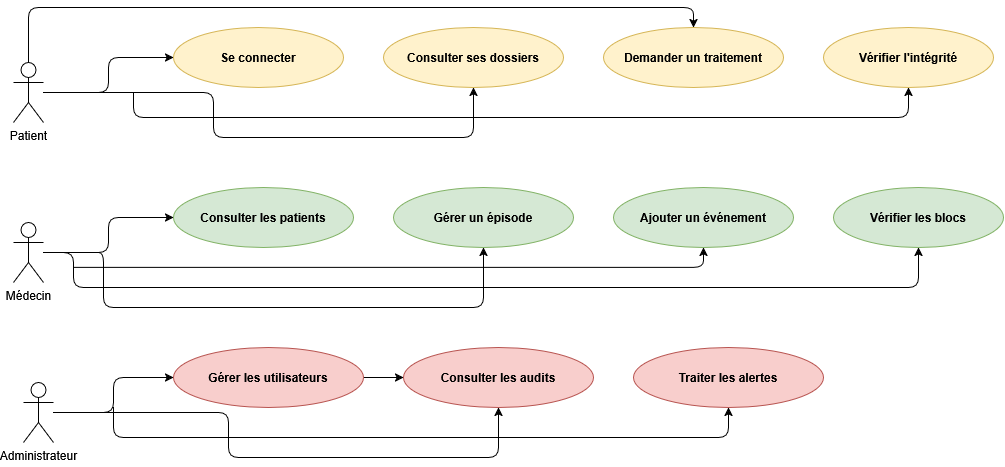
\includegraphics[width=\textwidth]{Chapters/2/images/02-cas-utilisation-global.png}
\caption{Diagramme de cas d'utilisation global}
\label{fig:use_case}
\end{figure}

\newpage 
\section{Besoins fonctionnels}

\subsection{Patient}

\begin{itemize}
    \item Créer un compte, se connecter et modifier son profil.
    \item Consulter la liste des médecins et prendre rendez-vous.
    \item Consulter ses dossiers médicaux.
    \item Demander un épisode de traitement et l'abandonner si nécessaire.
    \item Consulter la timeline de traitement et les détails d'intégrité.
\end{itemize}

\subsection{Médecin}

\begin{itemize}
    \item Consulter uniquement les épisodes de traitement dont il est le médecin.
    \item Activer un épisode demandé ou le clôturer.
    \item Créer des phases de traitement et ajouter des événements cliniques.
    \item Consulter l'état de vérification des blocs et des ancres.
\end{itemize}

\subsection{Administrateur}

\begin{itemize}
    \item Créer des utilisateurs, modifier leur rôle et activer ou désactiver un compte.
    \item Forcer la déconnexion d'un utilisateur.
    \item Consulter les indicateurs du tableau de bord.
    \item Consulter les journaux d'audit et traiter les alertes de sécurité.
\end{itemize}

\section{Besoins non fonctionnels}

\begin{itemize}
    \item \textbf{Confidentialité :} les charges utiles des événements cliniques sont chiffrées avec AES-GCM avant stockage.
    \item \textbf{Intégrité :} toute tentative de modification d'un bloc est rejetée ; les empreintes sont ancrées sur une chaîne EVM.
    \item \textbf{Traçabilité :} les connexions, consultations et refus d'accès sont enregistrés dans \texttt{AuditLog}.
    \item \textbf{Moindre privilège :} les requêtes sont filtrées selon le rôle et l'appartenance des données.
    \item \textbf{Disponibilité :} les services sont conteneurisés et supervisés par des healthchecks.
    \item \textbf{Maintenabilité :} la configuration sensible est externalisée dans l'environnement.
    \item \textbf{Sécurité des dépendances :} les versions sont épinglées dans \texttt{requirements.txt}.
\end{itemize}
\newpage
\section{Modèle de domaine}

La Figure \ref{fig:domain} présente les entités principales et leurs relations. Le cœur du modèle est l'épisode de traitement, auquel sont rattachés les phases, les événements cliniques, les blocs, la clé encapsulée et les ancres.

\begin{figure}[H]
\centering
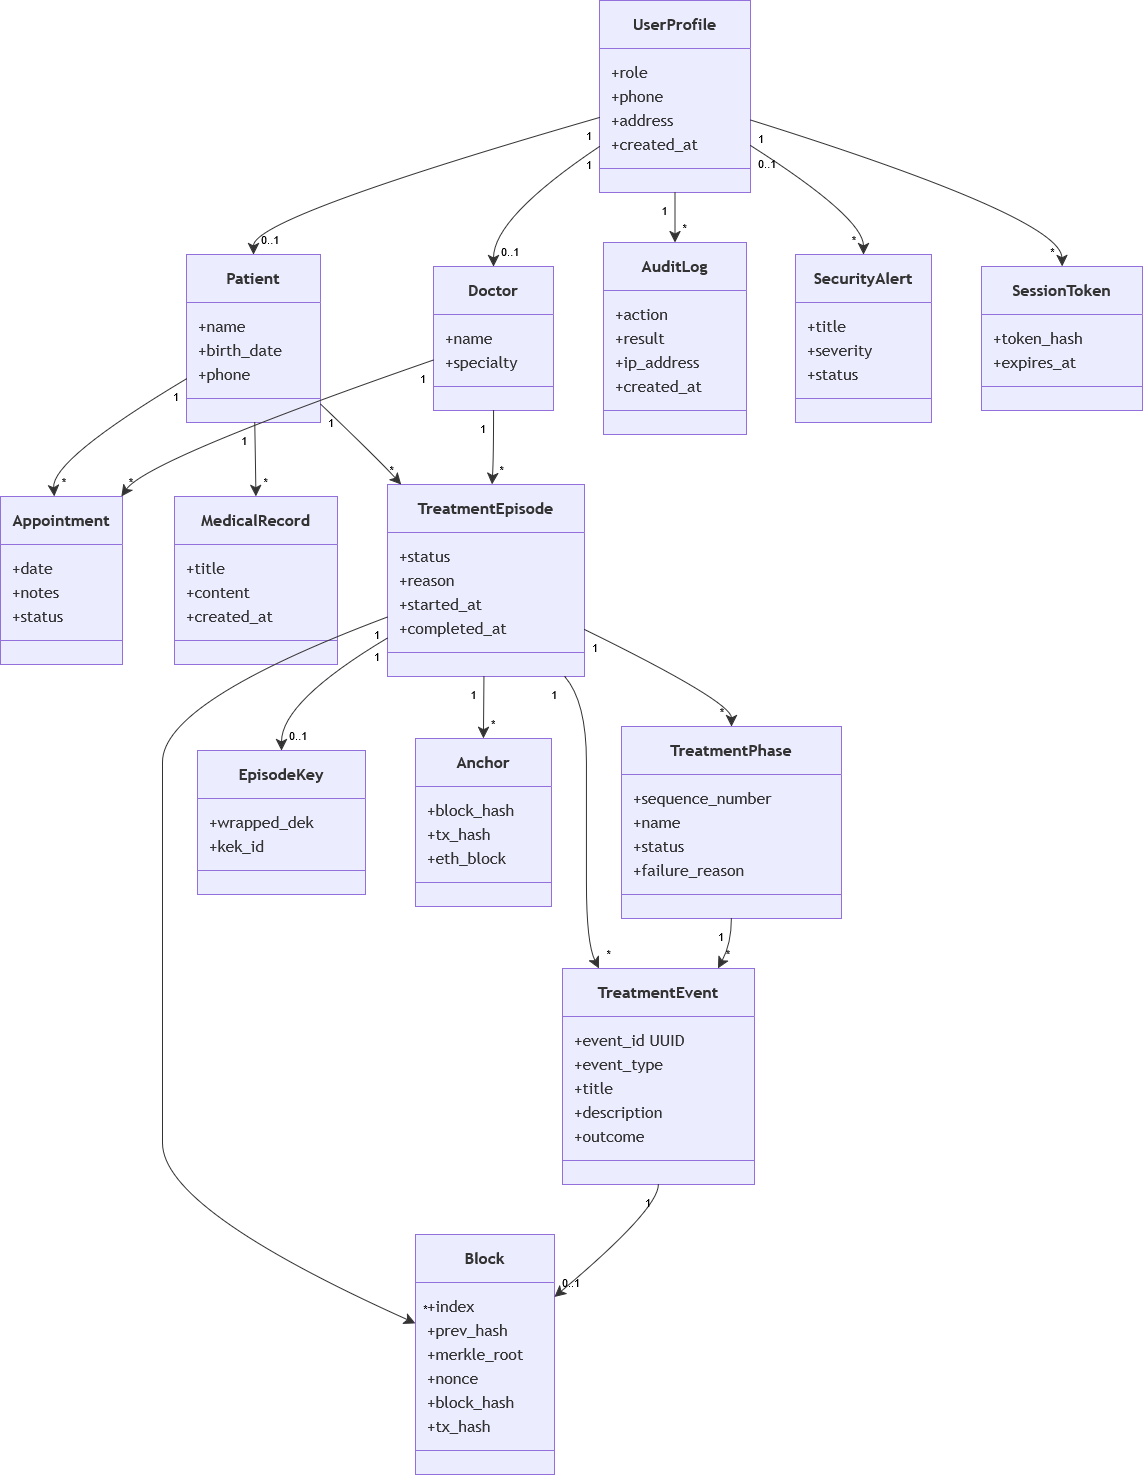
\includegraphics[width=\textwidth]{Chapters/2/images/05-modele-de-domaine.png}
\caption{Diagramme de classes du modèle de domaine}
\label{fig:domain}
\end{figure}
\newpage
\section{Architecture logicielle}

La Figure \ref{fig:backend_arch} décrit l'organisation en couches du backend : le middleware et le routage, les vues d'authentification, les vues métier et d'administration, les sérialiseurs, les modèles puis les services de stockage, de chiffrement et de journalisation.

\begin{figure}[H]
\centering
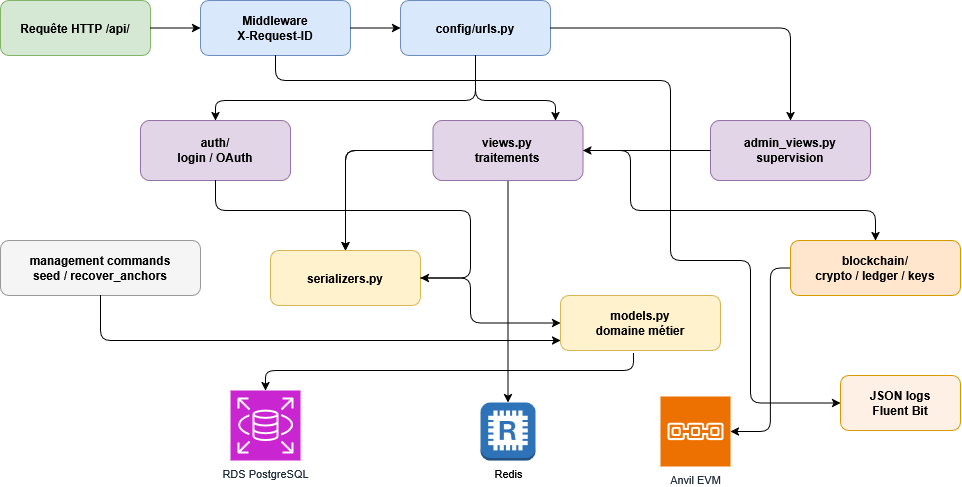
\includegraphics[width=\textwidth]{Chapters/2/images/04-architecture-backend.png}
\caption{Architecture en couches du backend}
\label{fig:backend_arch}
\end{figure}

La Figure \ref{fig:frontend_arch} décrit l'application monopage : les fournisseurs de contexte, le routeur, les pages publiques et protégées, puis la couche de services HTTP qui communique avec la passerelle.

\begin{figure}[H]
\centering
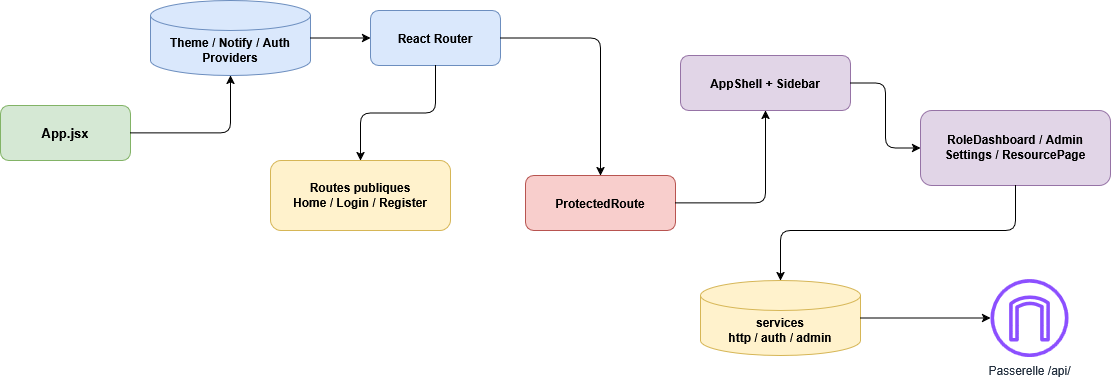
\includegraphics[width=\textwidth]{Chapters/2/images/12-architecture-frontend.png}
\caption{Architecture de l'application frontend}
\label{fig:frontend_arch}
\end{figure}

\section{Conclusion}

Les besoins et les modèles étant établis, les chapitres suivants détaillent les sprints de réalisation : authentification, parcours de soins, puis sécurité et déploiement.
